%%
%% 研究報告用スイッチ
%% [techrep]
%%
%% 欧文表記無しのスイッチ(etitle,eabstractは任意)
%% [noauthor]
%%

%\documentclass[submit,techrep]{ipsj}
\documentclass[submit,techrep,noauthor]{ipsj}



\usepackage[dvips]{graphicx}
\usepackage{latexsym}

\def\Underline{\setbox0\hbox\bgroup\let\\\endUnderline}
\def\endUnderline{\vphantom{y}\egroup\smash{\underline{\box0}}\\}
\def\|{\verb|}

%\def\newblock{\hskiip .11em plus .33em minus .07em}

%


%\setcounter{巻数}{59}%vol59=2018
%\setcounter{号数}{10}
%\setcounter{page}{1}


\begin{document}


\title{Code2Vec for C:C言語を対象としたコードの分散表現の獲得手法の提案}


\affiliate{IPSJ}{九州大学大学院 システム情報科学研究院\\
IPSJ, Faculty of Information Science and Electrical Engineering, Kyushu University}
\paffiliate{JU}{九州大学大学院 システム情報科学府\\
Graduate School of Information Science and Electrical Engineering, Kyushu University}
\paffiliate{F}{富士通九州ネットワークテクノロジーズ(株)\\
Fujitsu Kyushu Network Technologies Limited}

\author{檜枝 琴里}{Kotori Hieda}{JU}[hieda@f.ait.kyushu-u.ac.jp]
\author{久住 憲嗣}{Kenji Hisazumi}{IPSJ}[nel@slrc.kyushu-u.ac.jp]
\author{矢川 博文}{Hirofumi Yagawa}{F}
\author{福田 晃}{Akira Fukuda}{IPSJ}[fukuda@f.ait.kyushu-u.ac.jp]

\begin{abstract}
プログラムコードの分散表現を得るための手法としてCode2Vecが存在する.これはプログラムコードの埋め込みベクトルを得るために,メソッド本体などのコード片の機能を表すラベルを予測するタスクで学習するものである.これによりプログラムコードにおいてもコード片の意味を考慮した分散表現を得ることが出来る.Code2VecはJavaやC\#などのオブジェクト指向プログラムを対象としているが,組込みシステム開発ではオブジェクト指向言語ではないC言語を使用していることが多い.そのため,Code2Vecの手法を適用するために,C言語からの特徴量の抽出手法が必要であることや,関数名等の命名方法がオブジェクト指向言語と異なるためラベルの予測が困難といった課題がある.そこで本研究ではCode2Vecの手法をC言語プログラムにも対応可能にすべく,C言語からの特徴量の抽出手法を提案し,関数名等をオブジェクト指向言語と同様のモジュール名と機能名に分解するためのITF-DF手法を提案する.
\end{abstract}



\maketitle

%1
\section{序論}
自然言語処理ではWord2Vec\cite{rong2014word2vec}などの意味を考慮した分散表現を得る方法が提案されており様々な応用が展開している.プログラムコードにおいても同様の分散表現を得る手法を使用することにより,ソフトウェア開発を多様な側面から支援することができると考えられるが,手法,応用の両面ともに発展の余地がある.

プログラムコードの分散表現を得る手法としてCode2Vec\cite{alon2019code2vec}が提案されている.Code2Vecとはプログラムコードの分散表現を得るための手法のひとつであり,コード片を実数ベクトルとして表すことで,コード片やそれ同士の関連性を数値的に表現することができる.Code2Vecにより得られた分散表現を用いた主なタスクは,メソッド本体からのメソッド名の推定などがある.このCode2Vecは現状ではJavaやC\#等のオブジェクト指向プログラム言語を対象としている.しかしながら,組込みシステムなどで多く使用されているC言語はオブジェクト指向言語でないため,Code2VecをC言語にそのまま適用できない.特に関数名を推定するタスクにおいては,C言語の関数名がモジュール固有名と一般的な操作名との両者を含んでいるため,推定したい一般的な操作名のみの推定精度が低下する.

そこで本研究ではこの課題を解決すべく,ITF-DF(Inverse Term Frequency – Document Frequency)\cite{XXX}を関数名に適用する.ITF-DF手法とはある文書の中での出現頻度は低いが様々な文書を通して見ると出現頻度が高い単語の重要度が高くなるようにする指標とする.C言語の関数名にITF-IDF適用することにより,関数名を単語に分割した後にそれらをモジュール固有名と一般的な操作名とに選別する.そして,Code2Vecにおいて一般的な操作名のみを学習する.これにより,一つのプログラムコード内で頻繁に出てくる,それ特有でしかないモジュール固有名を削除し,広く一般的に使用される操作名のみを採用することを狙う.重要な操作名のみを関数名として学習することにより,関数名推定の精度向上を図る.

\begin{table}[t]
 \centering
 \caption{ITF-DF手法を用いた推定結果}
 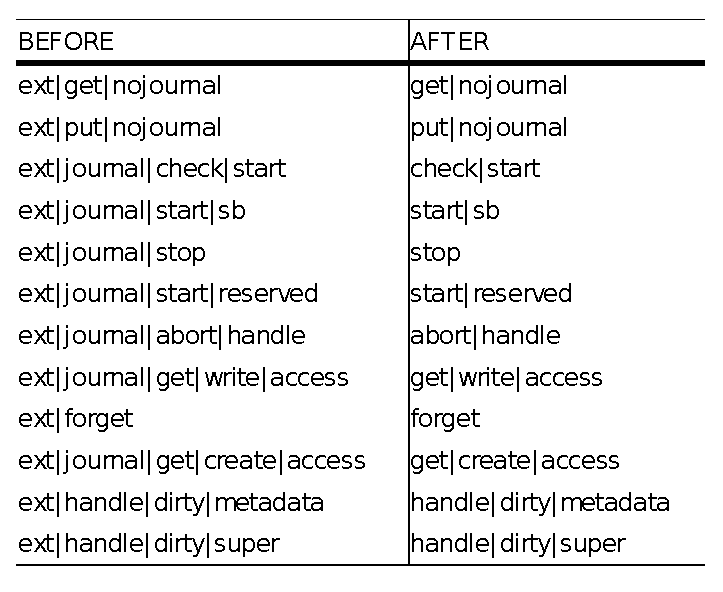
\includegraphics[width=1.0\hsize]{image/ITF-DFcompare.eps} 
 \label{table1} 
\end{table}

\section{関連研究}

% - code2vecの説明を節を分けてした方が良いと思います。code2vecの論文を見ながら概要を書いてもらうと良いと思いますが、特徴としては、従来はコードの構成要素のみを特徴量としていたのが、コードの終端記号と終端記号の間のパスを特徴量とすることで、コードの構造はほぼ同じだけれども細かい違いにより機能が変わるもの(配列の中からアイテムを取得する、配列の中にアイテムが存在するか?等)を見分けることが可能になったところかなと思います。
プログラムコードの分散表現を得る手法としてCode2Vec\cite{alon2019code2vec}が提案されている.従来手法では,プログラムコード中に出現する識別子等を学習し,分散表現を得ていた.しかしながらコード中の識別子はほぼ同様でありながらコードの機能が異なることがよくある.例えば,配列に対する操作において,配列中に指定した要素が存在するかどうかを判定するコードと,配列中に指定した要素があった場合にはその値を返すコードとは,ほぼ同じ構造であり返値が違うのみである.そこで,Code2Vecではこれらの細かな違いを分散表現に反映すべく,コードを抽象構文木にしたのち、木中のふたつの終端記号をつなぐ非終端記号や終端記号の列をパスとして抽出して特徴量とする.この特徴量に基づいて学習することにより,構造がほぼ同じでも細かい差により機能が変わるものを見分けることが可能となった.

%2
\section{解析手法}

本節ではC言語のプログラムコードを解析する手順を説明する.

C言語のプログラムは複数のファイルから構成されているが,ファイル毎に処理を行う.まず,関数の定義を抽出する.関数定義は関数名,引数,返値,関数本体から構成される.

関数名は通常複合語であるため,これから一般的な用語のみを抽出する.単語の区切りを表すために,単語の最初の文字を大文字にそれ以外を小文字にするキャメルケースや,\_が用いられるため,それらの区切りで単語を抽出する.さらに,数値は一般語のとしては不適切であることが多いため,数値を削除する.これを,用意した全てのC言語プログラミングコードのファイルを対象に行い,すべての単語についての出現文書数(DF)を計算し,全体の辞書とする.また,各ファイルごとに単語毎の出現頻度(TF)の辞書を作成する.これらの辞書に基づいてTF-IDFを計算する.文書Aにおける単語XのTF-IDFは,{log (文書Aにおける単語Xの出現頻度) / (文書Aにおける全単語の出現頻度の和)} * {(全文書数) / (単語Xを含む文書数)}で計算する.出現する全ての単語のTF-IDFを計算した後,閾値以下の単語を削除した関数名を作成する.

次に関数本体から特徴量を抽出する.Code2Vecの他言語用の実装に習って解析する.関数本体を構文解析して抽象構文木に変換し,木中の終端記号すべてを抽出する.抽出した終端記号のすべての組み合わせを作成する.組となる終端記号をつなぐ非終端記号や終端記号の列をパスとして抽出する.これを特徴量とする.

この一般語のみで構成した関数名と,関数本体から抽出した特徴量とをCode2Vecを用いて学習する.

% - 解析手法の節では、評価に関する記述はすべて除きます。代わりに特徴量の抽出手順を丁寧に説明します。また、clang/llvmなどの可能な限りプラットフォームなどの実装依存の説明と、アルゴリズムの説明を分離します。そして、まず一般性の高いアルゴリズムから説明します。できれば両者は小節を分けた方が良いでしょうね。

% 以下の手順を順に説明しましょう。
% 1) 関数名を_, camel case, 数値などで分割し、単語を抽出

% 2) すべてのファイルから単語を抽出して、TFやIDFを計算するための辞書を作成する

% 3) TF-IDFを計算し、閾値以下の単語を削除して推測したい関数名とする。

% この関数名を用いて学習し、この関数名を推定することとする。あとはcode2vecにまかせる。

% モジュール名と機能名に分類した関数名を,ITF-DF手法により{log (文書Aにおける単語Xの出現頻度) / (文書Aにおける全単語の出現頻度の和)} * {(全文書数) / (単語Xを含む文書数)} と計算し,ある文書の中での出現頻度は低いが様々な文書を通して見ると出現頻度が高い単語の重要度が高くなるように重み付けをした.さらにモジュール名と機能名に分類し重み付けをした関数名を,関数の内容と紐づけて学習した.これを辞書として用意し,関数の内容からその関数名として適切だと思われるものを,辞書から選び提案する.

\section{実装}

% 使用している環境の概要 pythonでlibclangでASTにして、ASTを探索することでパスを抽出している。
% libclangの説明 (書いてくれているこの文章はちょっと関係ないことまで書きすぎと思います。)
本研究では前節で説明した過程をPythonを用いて実装する.また,C言語を構文解析して抽象構文木にするために,clangを用いる.表XXに使用環境を示す.

% XXX表として,OS, Python version, clang versionなどをまとめた表を入れる.XXX

%ITF-DF手法を使って関数名などをモジュール名と機能名に分解して学習する.学習したらテストデータでうまくいくか試してみる.
%3
\section{結果}
関数名から一般名を抽出できているかを確認するために,実際のプログラムを対象にTF-IDFを計算し,閾値以下の単語を削除して関数名を再構成する.対象としたプログラムは linux 4.20 であり,逆文書頻度(IDF)はカーネル全体を対象として計算する.また、単語の出現頻度(TF)は fs/ext4/ext4_jbd2.c のみを対象として計算する.また,閾値は1.0とした.その結果を,表~\ref{table1}に示す.処理前の関数名は単語に分割したものを\|で結合した結果である.また,処理後はTF-IDFによる一般語抽出をした結果である.ITF-DFによる一般語抽出を実施する前はモジュール名が関数名に含まれるが,ITF-DF手法を用いることで,モジュール名を除外し,機能名のみを抽出することができた.
% 間違えてるのもあるけどなんとなくうまくいった.
% 〜〜(推定結果の図か表)〜〜

%4
\section{結論}
本研究ではCode2VecをC言語に適用すべく,LLVMとClangを用いて特徴量を抽出する実装について示した.また,関数本体から関数名を推定するタスクにおいては,C言語の関数名などの識別子は,モジュール名と一般的な機能名との複合語で構成されることが多いため,学習の際に障害になる可能性があることを議論した.さらに,この問題を解決すべく,C言語の関数名をTF-IDFを用いてモジュール名と機能名に分類する手法を提案した.その結果,C言語においても関数名から一般的な機能名のみを抽出することができることを示した.

今後の課題としては,提案手法を適用することにる評価,関数名のみではなく変数名等の多の識別子への適用による評価などが挙げられる.

% うまくいった.ラッキー.


% 謝辞
% \begin{acknowledgment}
% A4横型に対するガイドを基に,本稿を作成した.
% クラスファイルの作成においては,
% 京都大学の中島 浩氏にさまざまなご教示を頂き,
% さらにBiB\TeX 関連ファイルの利用についても快諾頂いたことを深謝する.
% また,A4横型に対するガイドを作成された当時の編集委員会の担当者に深謝する.
% \end{acknowledgment}


\bibliographystyle{ipsjunsrt}
\bibliography{bibsample}

% \begin{thebibliography}{10}

% \bibitem{webpage2}
% 情報処理学会論文誌ジャーナル編集委員会:
% べからず集(online),
% \urlj{http://www.ipsj.or.jp/journal/manual /bekarazu.html}
% (2011.09.15).

% \end{thebibliography}




\end{document}
